\section{Introducción}

En una economía con alta informalidad, un aumento del salario mínimo puede modificar tanto la remuneración de los trabajadores cubiertos como las oportunidades de acceder a un empleo formal. La evaluación requiere distinguir estas respuestas: un cambio pequeño del salario promedio puede coexistir con cambios en la composición del empleo, y una mayor participación del trabajo independiente no necesariamente implica que las mismas personas abandonaron puestos formales.

Este artículo estudia tres resultados alrededor de la reforma peruana de mayo de 2022: salario real por hora, formalidad y autoempleo. La Remuneración Mínima Vital (RMV) pasó de S/930 a S/1025, un incremento nominal de 10.2\%. Al tratarse de una política nacional, no existe un territorio sin reforma que funcione directamente como contrafactual. Comparo la evolución de trabajadores de baja educación, hasta secundaria completa, con la de trabajadores con alguna educación superior. Complemento ese contraste con la exposición regional previa al nuevo piso salarial, siguiendo la lógica de \citet{card_1992}.

La contribución consiste en examinar conjuntamente remuneración y composición del empleo en un episodio de recuperación pospandemia. El análisis se vincula con la evidencia peruana sobre salarios e informalidad de \citet{jaramillo_lopez_2006} y \citet{jimenez_2023}, y con el papel de la informalidad en la asignación del trabajo estudiado por \citet{ulyssea_2018}. La comparación entre grupos educativos es útil para medir cambios diferenciales, pero requiere separar la exposición al salario mínimo de otras diferencias en su recuperación económica.

Los resultados muestran una caída relativa de la formalidad y un aumento del autoempleo entre los ocupados de menor educación, sin una ganancia salarial relativa estadísticamente detectable. El gradiente regional presenta signos similares para la composición. Sin embargo, el contraste educativo es sensible a las tendencias previas, y el patrón de formalidad y autoempleo no se reproduce alrededor de la reforma de 2025. Estas reservas delimitan el alcance del resultado y motivan una interpretación prudente de su relación con la política.

\section{Contexto y datos}

La reforma entró en vigor el 1 de mayo de 2022 mediante el Decreto Supremo 003-2022-TR. La RMV del régimen general es nacional; sus efectos pueden diferir por la distribución salarial y el cumplimiento, aunque la fecha del cambio sea común. El trabajo por cuenta propia no recibe directamente un salario fijado por un empleador, pero puede responder a cambios en las oportunidades del trabajo asalariado. Por ello, la comparación incluye tanto el margen salarial como las proporciones de formalidad y autoempleo.

Utilizo los módulos trimestrales de empleo de la ENAHO entre 2021T1 y 2024T4. La muestra comprende personas de 14 a 65 años con educación válida. Excluyo 2022T2 porque mezcla observaciones anteriores y posteriores a la reforma; además, los ingresos se refieren al mes previo a la entrevista. La comparación utiliza cinco trimestres previos, 2021T1--2022T1, y diez posteriores, 2022T3--2024T4. La muestra general contiene 278\,064 observaciones, con tamaños menores para los resultados condicionados en empleo o salario válido.

El salario horario se calcula entre asalariados privados, incluidos trabajadores del hogar. Convierto los pagos diarios, semanales y quincenales a equivalentes mensuales, deflacto con el IPC de Lima del mes de referencia y divido por las horas mensuales de la ocupación principal. El resultado de regresión es su logaritmo, con la winsorización fijada en la preparación de la base. No incluye a quienes no perciben un salario válido ni mide su ingreso contrafactual si permanecieran asalariados.

Formalidad y autoempleo se definen entre ocupados no públicos. Formalidad identifica un empleo formal; autoempleo identifica a trabajadores por cuenta propia, excluyendo empleadores. Son dimensiones que pueden superponerse: un trabajador independiente puede ser formal. Sus coeficientes se presentan en puntos porcentuales de la población ocupada correspondiente, no de toda la población en edad de trabajar. El indicador de formalidad usa la clasificación oficial en 2021--2023 y una reconstrucción en 2024, un cambio de medición que limita la comparación temporal (Apéndice~\ref{app:short_measure}).

La baja educación corresponde a secundaria completa o menos, códigos 1--6 de \texttt{p301a}; la alta educación, a alguna educación superior, códigos 7--11. La educación especial y los valores faltantes se excluyen. Esta clasificación aproxima diferencias de exposición, pero no asigna jurídicamente el tratamiento. Los años educativos empleados como control son valores imputados a cada categoría, no una medición continua de años aprobados.

\section{Estrategia empírica}

\subsection{Contraste educativo y dinámica temporal}

Para el individuo $i$, departamento $r$ y trimestre $t$, estimo
\begin{equation}
Y_{irt}=\alpha_r+\lambda_t+\gamma L_i+\beta(L_iP_t)+X_i'\delta+\varepsilon_{irt},
\label{eq:short_did}
\end{equation}
donde $L_i$ indica baja educación y $P_t$ el período posterior. El vector $X_i$ contiene edad, edad al cuadrado, sexo, estado civil, zona urbana y años educativos imputados. Los efectos fijos de trimestre absorben cambios nacionales comunes y los de departamento, diferencias territoriales persistentes. Pondero con \texttt{fac500a} y agrupo los errores por departamento, con 25 grupos.

El coeficiente $\beta$ mide cuánto cambió el resultado del grupo de baja educación respecto del cambio del grupo de alta educación, condicional en esos controles. Una interpretación causal requiere que, sin la reforma, ambos grupos habrían seguido tendencias paralelas y que no existan shocks diferenciales coincidentes. Como el grupo de alta educación también puede verse afectado, el contraste no identifica automáticamente el efecto absoluto de la RMV sobre el grupo de baja educación. Tampoco se presupone que esa exposición compartida produzca necesariamente una atenuación hacia cero.

Estimo además un estudio de eventos que reemplaza $L_iP_t$ por interacciones de $L_i$ con cada trimestre, omitiendo 2022T1. Los coeficientes previos permiten evaluar la compatibilidad de los datos con tendencias paralelas; los posteriores describen la evolución de la brecha ajustada. No rechazar una prueba previa es informativo, pero no demuestra el supuesto de identificación \citep{roth_2022_pretest}.

\subsection{Exposición regional complementaria}

El segundo diseño reemplaza el contraste educativo por la intensidad regional previa:
\begin{equation}
Y_{irt}=\mu_r+\eta_t+\theta(P_tK_r)+X_i'\pi+u_{irt}.
\label{eq:short_regional}
\end{equation}
El índice $K_r$ es el cociente entre S/1025 y la mediana salarial mensual nominal previa de los asalariados privados del departamento, estandarizado entre los 25 departamentos. Una unidad representa una desviación estándar de esa distribución regional. Uso las mismas muestras de resultados y controles; el modelo no incluye por separado el indicador de educación baja.

El coeficiente $\theta$ describe el cambio posterior asociado con una mayor exposición regional previa. Este diseño ofrece una comparación adicional, con otro supuesto: en ausencia de la reforma, la evolución de los resultados no debería depender sistemáticamente de $K_r$, condicional en los controles. Medir el índice antes del cambio evita construirlo con resultados posteriores, pero no hace exógena la exposición. Las regiones de salarios bajos podrían experimentar recuperaciones o shocks distintos. Por ello, la coincidencia de signos entre los dos diseños es evidencia complementaria y no una validación automática de causalidad.

\section{Resultados}

\subsection{Salarios y composición del empleo}

El Cuadro~\ref{tab:short_main} concentra los tres resultados. El salario horario relativo cambia $-0.021$ log puntos ($p=0.106$), aproximadamente $-2.04\%$. El intervalo convencional al 95\% equivale aproximadamente a $[-4.50\%,\,0.47\%]$. No se detecta una ganancia salarial relativa al 5\%, pero esta estimación no demuestra que el efecto sea cero y su interpretación depende de las tendencias previas.

La proporción de empleo formal cae 4.64 puntos porcentuales y la de autoempleo aumenta 3.63 puntos entre los ocupados no públicos de baja educación, respecto de los de alta educación. Ambas estimaciones son significativas con los errores agrupados convencionales. Son cambios de composición en cortes transversales: no establecen, por sí solos, que los mismos trabajadores pasaron de empleos formales al autoempleo.

\begin{table}[!htbp]\centering
\caption{Tres resultados centrales del contraste educativo}\label{tab:short_main}
\begin{threeparttable}\small
\setlength{\tabcolsep}{4pt}
\begin{tabular}{lrrrrr}
\toprule
Resultado & $N$ & DiD & IC 95\% & $p$ & $p$ previo \\
\midrule
Salario horario (log) & 69,534 & -0.021 & [-0.046, 0.005] & 0.106 & 0.001 \\
 &  & (0.012) &  &  &  \\
Formalidad (pp) & 181,317 & -4.642 & [-6.167, -3.117] & $<0.001$ & 0.148 \\
 &  & (0.739) &  &  &  \\
Autoempleo (pp) & 181,317 & 3.630 & [2.402, 4.859] & $<0.001$ & 0.003 \\
 &  & (0.595) &  &  &  \\
\bottomrule
\end{tabular}
\begin{tablenotes}\footnotesize
\item Coeficiente de baja educación por período posterior de la ecuación~\eqref{eq:short_did}. ENAHO 2021T1--2024T4, sin 2022T2. Salarios: asalariados privados con remuneración horaria válida. Formalidad y autoempleo: ocupados no públicos. Los indicadores binarios se expresan en puntos porcentuales (pp). Errores agrupados por departamento entre paréntesis; 25 grupos, ponderadores de encuesta. IC con distribución $t_{24}$. La última columna contrasta conjuntamente los coeficientes previos del estudio de eventos; no rechazar no demuestra tendencias paralelas.
\end{tablenotes}
\end{threeparttable}\end{table}


La Figura~\ref{fig:short_event} muestra la trayectoria de estas brechas. La prueba conjunta previa rechaza para salarios ($p=0.001$) y autoempleo ($p=0.003$), mientras que para formalidad no rechaza ($p=0.148$). En consecuencia, la significación de los coeficientes posteriores no basta para atribuirlos a la reforma. Las diferencias de precisión entre resultados tampoco sustituyen una evaluación de sus supuestos.

\begin{figure}[!htbp]
\centering
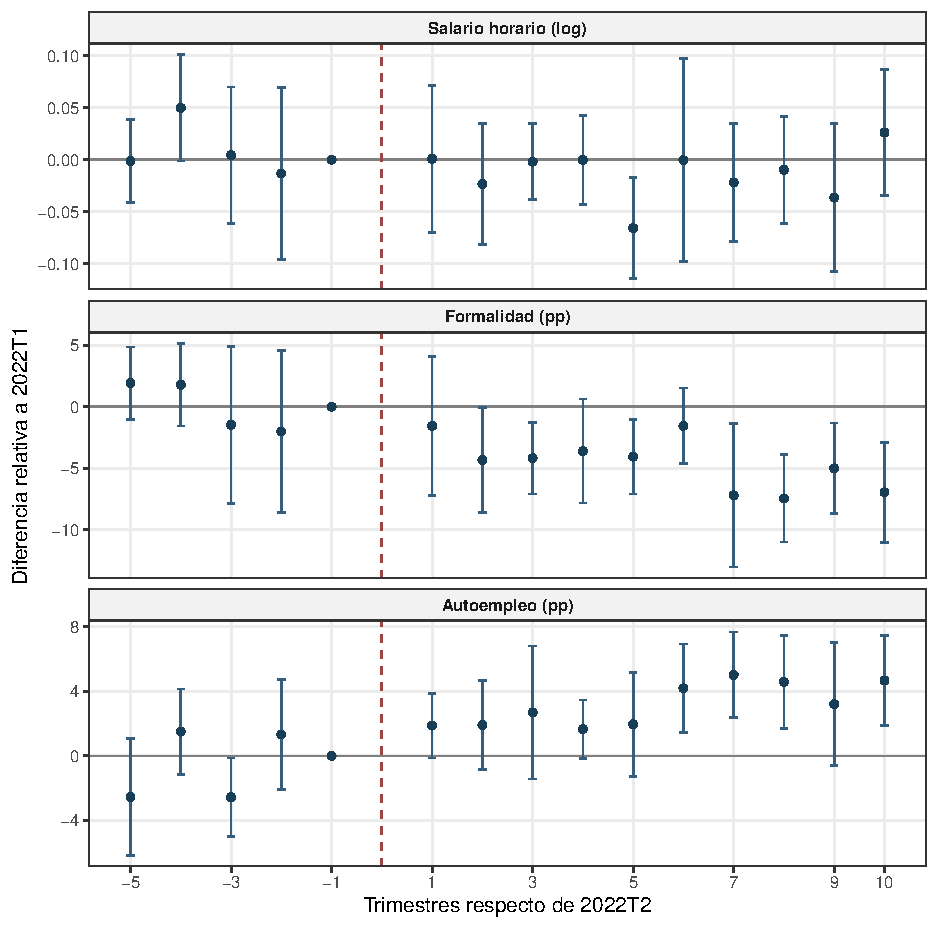
\includegraphics[width=.95\textwidth]{paper/espanol_corta/figures/eventos_tres_resultados.pdf}
\caption{Dinámica de los tres resultados respecto de 2022T1}
\label{fig:short_event}
\begin{minipage}{.95\textwidth}\footnotesize
Notas: Interacciones de baja educación por trimestre, con los controles de la ecuación~\eqref{eq:short_did}. El trimestre de referencia ($k=-1$) está normalizado a cero; 2022T2 ($k=0$) se excluye. Intervalos al 95\% con errores agrupados por departamento y valor crítico $t_{24}$. Las escalas verticales difieren: salarios en log puntos; formalidad y autoempleo en puntos porcentuales.
\end{minipage}
\end{figure}

El diseño regional estima una caída de 1.83 puntos en formalidad y un aumento de 1.00 punto en autoempleo por cada desviación estándar adicional de exposición (Cuadro~\ref{tab:short_regional}). La asociación salarial es positiva, $0.017$ log puntos, e imprecisa con errores agrupados ($p=0.154$). Las pruebas previas regionales no rechazan para ninguno de estos tres resultados. La evidencia regional acompaña el patrón de composición, pero no reproduce una caída salarial precisa ni elimina la posibilidad de shocks correlacionados con el nivel salarial inicial.

\begin{table}[!htbp]\centering
\caption{Cambios asociados con la exposición regional previa}\label{tab:short_regional}
\begin{threeparttable}\small
\setlength{\tabcolsep}{4pt}
\begin{tabular}{lrrrr}
\toprule
Resultado & Coeficiente & EE & $p$ & $p$ previo \\
\midrule
Salario horario (log) & 0.017 & 0.012 & 0.154 & 0.243 \\
Formalidad (pp) & -1.827 & 0.346 & $<0.001$ & 0.842 \\
Autoempleo (pp) & 1.003 & 0.400 & 0.019 & 0.202 \\
\bottomrule
\end{tabular}
\begin{tablenotes}\footnotesize
\item Coeficiente de período posterior por índice de Kaitz estandarizado, ecuación~\eqref{eq:short_regional}. Una unidad equivale a una desviación estándar entre los 25 departamentos. Misma ventana, muestras de resultados, controles individuales y ponderadores que en el Cuadro~\ref{tab:short_main}. El modelo regional no incluye el indicador binario de educación baja. Errores agrupados por departamento. Los valores $p$ previos corresponden a adelantos de exposición regional. No se mezclan aquí con valores $p$ de modelos colapsados o permutados.
\end{tablenotes}
\end{threeparttable}\end{table}


\subsection{Entrada a la formalidad y comparación con 2025}

Para examinar el margen de ajuste, utilizo como complemento los resultados del Panel ENAHO 2020--2024. Apilo pares de años consecutivos y comparo transiciones de trabajadores de baja y alta educación con efectos fijos de par y departamento, controles demográficos y ponderadores de panel. Entre quienes partían de la informalidad, la entrada a un empleo privado formal se reduce 2.12 puntos porcentuales en los pares posteriores a la reforma ($p=0.011$), frente a una tasa previa de 4.51\% para el grupo de baja educación.

Entre quienes ya eran formales, la permanencia relativa aumenta 8.26 puntos en los pares que cruzan la reforma ($p=0.055$), pero la estimación para los pares posteriores es $-2.23$ puntos y no es significativa ($p=0.310$). El panel es compatible con una menor entrada posterior a la formalidad; no permite afirmar que no hubo salidas ni que ese margen explique toda la caída observada en los cortes transversales. Su frecuencia anual, el punto de partida pandémico de algunos pares y las 7011 observaciones de base formal aconsejan tratarlo como evidencia sugerente del mecanismo.

El contraste con la reforma de enero de 2025 acota la generalización. Al replicar el diseño educativo en 2024--2025, el coeficiente salarial es $0.002$ log puntos y el de formalidad, $-0.07$ puntos porcentuales, ambos imprecisos. El autoempleo disminuye 1.43 puntos ($p=0.026$), de signo opuesto a 2022 (Cuadro~\ref{tab:short_2025}). Los dos episodios difieren en su contexto y en la distribución salarial inicial; esta comparación no identifica cuál diferencia explica el resultado. Sí muestra que el patrón de composición de 2022 no se reproduce de forma estable en el segundo episodio.
\FloatBarrier

\section{Credibilidad y alcance}

La limitación principal del contraste educativo es distinguir el cambio asociado con la reforma de una evolución diferencial preexistente. El análisis de sensibilidad de \citet{rambachan_roth_2023} incluye cero en los intervalos de formalidad y autoempleo al permitir desviaciones posteriores de magnitud relativa $\bar M=0.1$. Este ejercicio se aplica al promedio de coeficientes posteriores del estudio de eventos, no exactamente al mismo estimando ponderado del coeficiente estático. En conjunto con las pruebas previas, indica que las conclusiones causales requieren restricciones fuertes sobre las tendencias contrafactuales.

Las variantes rutinarias preservan los signos de composición, pero algunas alternativas cambian sustancialmente el resultado. Una tendencia lineal específica por grupo educativo reduce las estimaciones a $-0.35$ puntos en formalidad y $+0.61$ en autoempleo, ambas imprecisas. Puede absorber una deriva o parte de un cambio persistente; no es posible resolver esa ambigüedad declarando que la especificación es demasiado exigente. El estimador doblemente robusto y la corrección CR2 sobre datos colapsados también reducen la precisión. El Apéndice~\ref{app:short_robustness} presenta estas discrepancias junto con las variantes favorables, en lugar de resumirlas como estabilidad general.

La exposición regional enfrenta una amenaza distinta: la crisis política y la recesión se superponen con parte de la ventana posterior. Los controles de protestas y las exclusiones geográficas del análisis complementario mantienen un gradiente negativo de formalidad. Sin embargo, al limitar la ventana posterior a 2022T3--T4, la pendiente se reduce a $-0.61$ puntos y pierde significación ($p=0.113$). Ese tramo tampoco está completamente libre de crisis, que comienza en diciembre de 2022. La evidencia regional es más clara para el período posterior amplio que para el ajuste inmediato; controlar una dimensión del conflicto no descarta todos los shocks regionales concurrentes.

La selección y la medición son igualmente relevantes. Los salarios se observan para quienes permanecen asalariados con remuneración válida. Formalidad y autoempleo dependen del denominador de ocupados, que puede variar. En la especificación regional que usa toda la población en edad de trabajar como denominador, el empleo formal cae 1.62 puntos por desviación estándar de exposición, pero el autoempleo no aumenta: su coeficiente es $-0.44$ puntos ($p=0.100$). Por tanto, una mayor participación del autoempleo entre los ocupados no demuestra una expansión de su nivel absoluto. El empalme del indicador de formalidad en 2024 añade otra fuente de incertidumbre.

Finalmente, agrupar errores por departamento permite correlación dentro de cada grupo, pero no convierte la comparación nacional entre dos grupos educativos en una asignación aleatoria de tratamiento. Los valores $p$ deben leerse condicionales al modelo y al esquema de inferencia. La cantidad de observaciones individuales no elimina por sí sola las limitaciones del diseño.

\section{Conclusiones}

Alrededor de la reforma de 2022 se observa una reducción relativa de la formalidad y un aumento de la participación del autoempleo entre los ocupados de menor educación, sin una ganancia salarial relativa estadísticamente detectable. La exposición regional presenta asociaciones de composición del mismo signo, mientras que el panel anual sugiere una menor entrada posterior a la formalidad. Estas piezas describen dimensiones diferentes del ajuste y no deben interpretarse como estimaciones intercambiables de un mismo efecto causal.

Las tendencias previas, la sensibilidad a su relajación, la composición de las muestras y el contraste con 2025 limitan una conclusión general sobre el salario mínimo. La evidencia justifica prestar atención al acceso a empleos formales además de la remuneración, pero no permite afirmar que cualquier aumento de la RMV provoque informalización o carezca de beneficios salariales. Una identificación más convincente del mecanismo requeriría datos de transiciones de mayor frecuencia y una fuente de variación de exposición menos ligada a la recuperación económica regional o educativa.
